%%%%%%%%%%%%%%%%%%%%%%%%%%%%%%%%%%%%%%%%%%%%%%%%%%%%%%%%%%%%%%%%%%% 
%                                                                 %
%                            CHAPTER                              %
%                                                                 %
%%%%%%%%%%%%%%%%%%%%%%%%%%%%%%%%%%%%%%%%%%%%%%%%%%%%%%%%%%%%%%%%%%% 

\chapter{Software implementation with pure Smith-Waterman}

This capter will cover an approach to reference genome mapping using pure smith-waterman. This is a computationally very demanding task, but is more precise than heuristic methods such as FASTA, ...

\section{The concept}
For reference genome mapping a sequence of 100 to 1000 bases in length should be mapped to the reference genome. The idea behind this mapping and the applications is thouroughly described in \ref{ch:algoverzicht}.

In this implementation, a mapping with "pure" Smith-Waterman was chosen. Commonly, an algorithm is used to select canditate locations where a small local smith-waterman is performed, or no smith waterman is performed at all. These methods are often less precise but computationally less demanding. Here, the alignment of the sequence is done with the full reference genome.

 //figuurtje


\section{General overview of the implementation}

\subsection{Parameters and Types}

\paragraph{Nucleotide base}
First of all, It seemed important to define the nucleotide bases. There are only 4 possible bases ($A$, $C$, $G$ and $T$), so 2 bits are enough. The following coding was chosen:

\begin{table}[H]
	\centering
	\begin{tabular}{|l|c|c|c|c|}
		\hline
		\textbf{Base} & A  & C  & G  & T  \\ \hline
		\textbf{Code} & 00 & 01 & 10 & 11 \\ \hline
	\end{tabular}
	\caption{\centering Encoding for the nucleotide bases}
\end{table}

To store these bases the uint8\_t type type from the stdint library was used. it is 1 byte in size which is the smallest available type in the C language. If more time would have been available, and an implementation with the full human genome would have been made, it might be a good idea to define a specific type consisting of only 2 bits, which would be a lot more memory efficient.

\paragraph{DNA sequence type}

store string of DNA 
struct: length + pointer to first element
types for the index: Ref and Seq

\subsection{The code structure}

\begin{enumerate}
	\item reserve memory for:
	\begin{enumerate}
		\item genome
		\item current read
		\item reverse of current read
		\item matrix for during the alignment
	\end{enumerate}
	\item initialize the first row and first column of the matrix on $0$
	\item load the genome from file
	\item open the FASTQ (for loading unmapped reads) and SAM (for storing mapped reads) file
	\item for every read in the FASTQ file:
	\begin{enumerate}
		\item load the next read from FASTQ file
		\item perform the alignment. This is the most computationally demanding step.
		\item write the mapped read to the SAM file
	\end{enumerate}
	\item close the open FASTQ and SAM file
	\item free the reserved memory again
\end{enumerate}

\section{Details of the implementation}

splitting up the problem.

\begin{figure}[H]
	\centering
	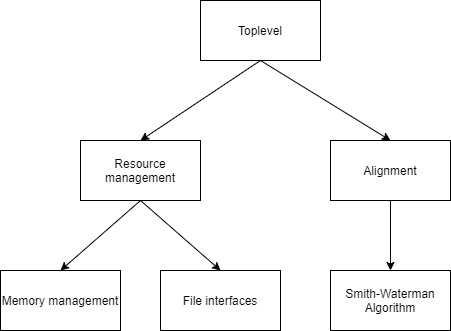
\includegraphics[width=0.5\textwidth]{systemImplementation/organigram.png}
	\caption{an organisation chart of the split up functionalities}
	\label{fig:organigram}
\end{figure}

\subsection{File Interfaces}

types!

Conversion functions char -> base and base -> char

FASTA interface => loads genome:
splitting functions
Genome info
Putting Reference info into array

FASTQ interface => loading next read (stream)
splitting functions
get qname
get sequence
get qualities

SAM interface 
init for the defaults (Rnext, Pnext, Tlen)
writeSAMline => writes the mapped read in the sam file in the right format


\subsection{Memory Management}

sdsalloc VS malloc
choosing sdsalloc so that hardware can also get it easily

\subsection{The alignment}

computational complexity: O(mn)

\section{Implementation results}

\subsection{Sample data}

PhiX 
galaxy
FASTQ: https://github.com/Illumina/Isaac3/tree/master/src/data/examples/PhiX/Fastq
coronavirus

//figuurtje IGV
uitleggen reading depth + sequence direction
desired result

\subsection{Results}

//figuurtje + bespreking
